\documentclass{beamer}
\usetheme{Madrid}
\useinnertheme{circles}
\addtobeamertemplate{footnote}{}{\vspace{1.5ex}}
\definecolor{UBCblue}{rgb}{0.04706, 0.13725, 0.26667} % UBC Blue (primary)
\hypersetup{linkcolor=}
\usecolortheme[named=UBCblue]{structure}
\setbeamercolor{title in head/foot}{fg=white}
\title[]{Scattering Observables from Few-Body Densities and Application in Light Nuclei }
\author{Alexander Long}
\institute[GWU]{George Washington University - Washington DC USA}
\date{\parbox{\linewidth}{
  \centering
  Support from the US Department of Energy\endgraf
  In collaboration with:\endgraf Harald Griesshammer, Andreas Nogga, Xiang-Xiang Sun  \endgraf\par
  }}
\usepackage{bigints} 
\usepackage{listings}
\usepackage{feynmp-auto} % mpost afilename
\DeclareGraphicsRule{*}{mps}{*}{} % for being able to read the produced file

\usepackage{amsmath}
\usepackage{mathtools}
\usepackage{mathrsfs}
\usepackage[style=british]{csquotes}
% \usepackage[]{graphicx}
\usepackage{slashed}
\usepackage{mathrsfs}
\usepackage[normalem]{ulem}
\usepackage{outlines}
\usepackage{tikz}
\usepackage{bbm}
\usepackage{wrapfig}
% \usepackage[backend=biber,citestyle=alphabetic,style=numeric]{biblatex}
% \addbibresource{refs.bib}
% \AtBeginBibliography{\tiny}
\def\checkmark{\tikz\fill[scale=0.4](0,.35) -- (.25,0) -- (1,.7) -- (.25,.15) -- cycle;} 
\newcommand{\s}{\slashed}
\newcommand{\p}{\partial}

\usepackage{mathrsfs}  
\newcommand{\Lscr}{\mathscr{L}}

\newcommand\ddfrac[2]{\frac{\displaystyle #1}{\displaystyle #2}}
\DeclarePairedDelimiter\br{\langle}{\rvert}
\DeclarePairedDelimiter\kt{\lvert}{\rangle}
\DeclarePairedDelimiterX\brkt[2]{\langle}{\rangle}{#1 \delimsize\vert #2}
\newcommand\brktt[3]{\left< #1 \right| #2 \left| #3 \right>}

\newcommand{\D}{\Theta}
\newcommand{\He}{\mathrm{He}}
\newcommand{\Li}{\mathrm{Li}}
\newcommand{\LiS}{{}^{6} \mathrm{Li} }
\newcommand{\HeF}{{}^{4} \mathrm{He}}
\newcommand{\HeT}{{}^{3} \mathrm{He}}
\newcommand{\HT}{{}^{2} \mathrm{H}}
\newcommand{\bv}{\vec}
\newcommand{\e}{\mathrm{e}}
\newcommand{\dd}{\mathrm{d}}
\newcommand{\deint}[2]{\dd^{#1}\;\!\!#2\;}
\newcommand{\jrel}{\ensuremath{j_{12}}}
\newcommand{\ev}{\vec{e}}
\newcommand{\kv}{\vec{k}}
\newcommand{\pv}{\vec{p}}%{\vec{\,\!p}\!\:{}}
\newcommand{\qv}{\vec{q}}%{\vec{\,\!q}\!\:{}}
\newcommand{\xv}{\vec{x}}
\newcommand{\yv}{\vec{y}}
\newcommand{\bra}{\langle}
\newcommand{\ket}{\rangle}

\newcommand\footn[1]{%
  \begingroup
  \renewcommand\thefootnote{}\footnote{#1}%
  \addtocounter{footnote}{-1}%
  \endgroup
}

\newcommand{\sepp}{,}
\newcommand{\sep}{}

\newcommand{\hqm}{\hspace*{-0.25em}}
\newcommand{\hqmm}{\hspace*{-0.5em}}
\newcommand{\hqmmm}{\hspace*{-1.0em}}
% \newcommand\ot[1]{{#1}_{12}}
\newcommand\ot{_{12}}
\hypersetup{
    colorlinks,
    citecolor=blue,
    filecolor=black,
    linkcolor=blue,
    urlcolor=black
}

 \usepackage[english]{babel}
\usefonttheme{serif} % default family is serif
\newcommand{\bs}{\boldsymbol}

\setbeamerfont{frametitle}{size=\Large}
\setbeamerfont{framesubtitle}{size=\Large}
\begin{document}
\setbeamertemplate{itemize items}[triangle]
\setbeamertemplate{enumerate items}[default]

\titlepage


\begin{frame}{1. Introduction}{Motivation}
\underline{Transition Density Method}: \\~\\
Factor into probe interaction with active nucleons (kernel) and spectator nucleon behavior (density)\\~\\
Allows interaction kernel to be recycled for different targets\\~\\
Allows nucleus description to be recycled for different interactions\\~\\
Allows code to be recycled for different interactions and nuclei
\footn{``Scattering Observables from One- and Two-Body Densities Griesshammer et. al. \href{https://arxiv.org/abs/2005.12207}{arXiv:2005.12207}}
\end{frame}
%%%%%%%%%%%%%%%%%%%%%%%%%%%%%%%%%%%%%%%%%%%%%%%%%%%%%%%%%%%%%%%%%%%%%%%%%%%%%%%%%%%%%%%%%%%%%%%%%%%




\begin{frame}{Overview}
\begin{center}
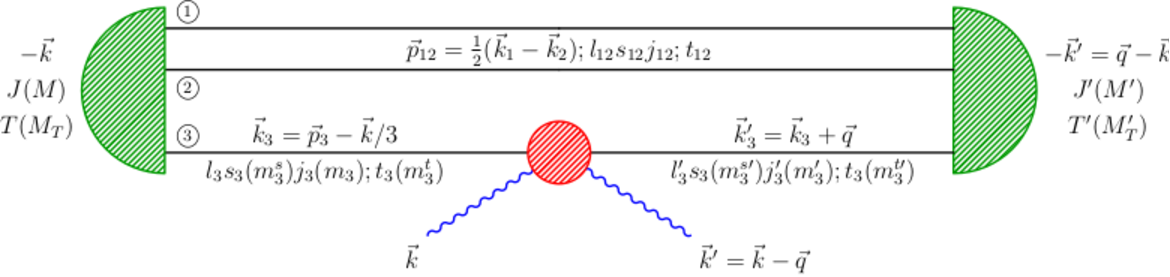
\includegraphics[scale=0.07]{kinematics3He-1bod.png}
\end{center}
    Probe interacts with $n$ active nucleons $\implies$ \textit{$n$ body kernel} $\implies$ \textit{$n$ body transition density}.
Density independent of probe, kernel independent of density\\~\\
Transition density $\rho$ is the probability amplitude of a nucleus with quantum numbers $\kt{M_J}$ to absorb the momentum $\vec{q}=\vec{k}_2-\vec{k}_1$ and change into quantum numbers $\kt{M_J'}$
\end{frame}
%%%%%%%%%%%%%%%%%%%%%%%%%%%%%%%%%%%%%%%%%%%%%%%%%%%%%%%%%%%%%%%%%%%%%%%%%%%%%%%%%%%%%%%%%%%%%%%%%%%


\begin{frame}\frametitle{}
\begin{figure}[ht]
\begin{center}
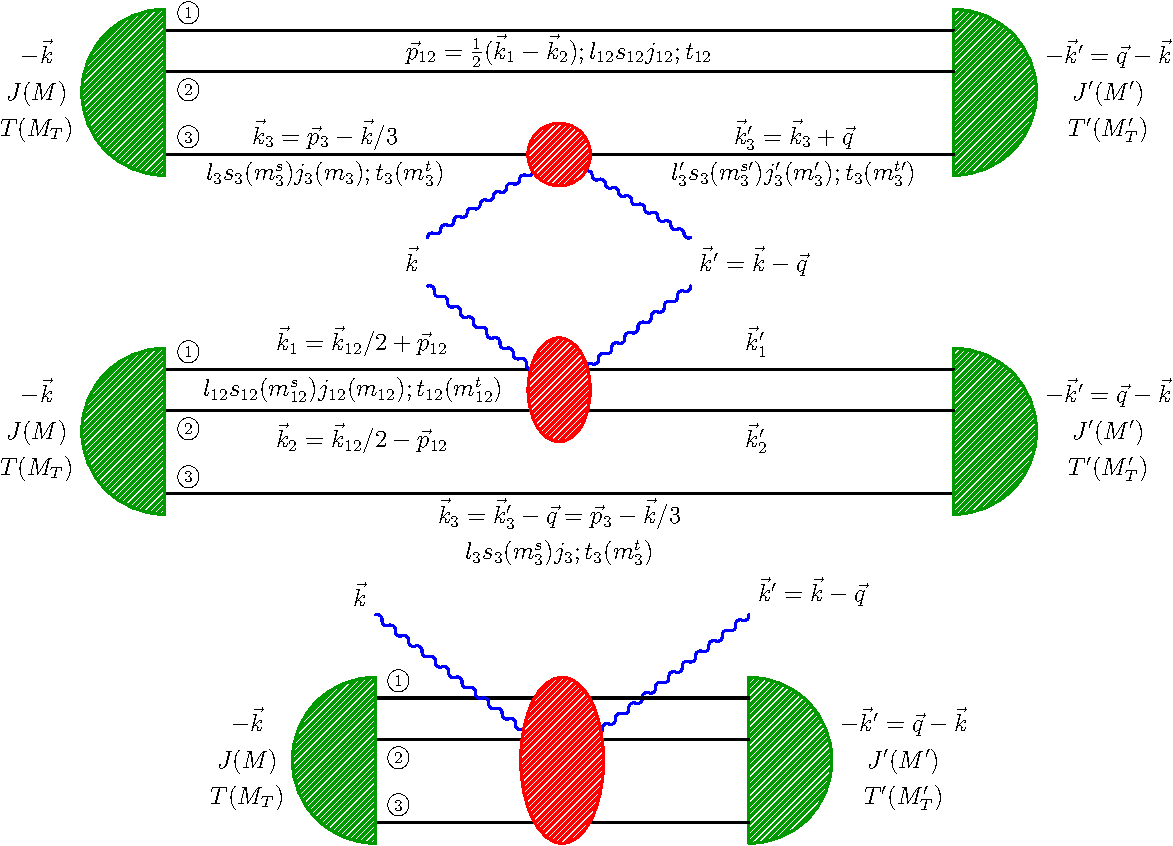
\includegraphics[scale=0.50]{kinematics3He.pdf}
\caption{Griesshammer/... Few-B Sys 61 (2020) 48}
\end{center}
\end{figure}
\end{frame}
%%%%%%%%%%%%%%%%%%%%%%%%%%%%%%%%%%%%%%%%%%%%%%%%%%%%%%%%%%%%%%%%%%%%%%%%%%%%%%%%%%%%%%%%%%%%%%%%%%%

\begin{frame}{Total Contribution}
For an $n$ body system, total scattering amplitude is:
\begin{align*}
    A_{M}^{M^{\prime} }(\bv{k}, \bv{q})&=\binom{A}{1}\left\langle M^{\prime}\right|\hat{O}_{3}^{}(\bv{k}, \bv{q})\left|M\right \rangle + \binom{A}{2} \left\langle M^{\prime}\right|\hat{O}_{12}^{}(\bv{k}, \bv{q}) \left| M\right\rangle\\
        &+ \binom{A}{3}\left\langle M^{\prime}\right|\hat{O}_{123}^{}(\bv{k}, \bv{q})\left|M\right \rangle + \binom{A}{4} \left\langle M^{\prime}\right|\hat{O}_{1234}^{}(\bv{k}, \bv{q}) \left| M\right\rangle\\
        &+... + \binom{A}{A}\left\langle M^{\prime}\right|\hat{O}_{1...A}^{}(\bv{k}, \bv{q})\left|M\right \rangle
\end{align*}
$\binom{A}{i}$ ways to hit $i$ nucleons in a nucleus with $A$ nuclei
\end{frame}
%%%%%%%%%%%%%%%%%%%%%%%%%%%%%%%%%%%%%%%%%%%%%%%%%%%%%%%%%%%%%%%%%%%%%%%%%%%%%%%%%%%%%%%%%%%%%%%%%%%



\begin{frame}{Truncated Result}
We use only the first two terms
\begin{equation*}
    A_{M}^{M^{\prime} }(\bv{k}, \bv{q})=\binom{A}{1}\left\langle M^{\prime}\right|\hat{O}_{3}^{}(\bv{k}, \bv{q})\left|M\right \rangle + \binom{A}{2} \left\langle M^{\prime}\right|\hat{O}_{12}^{}(\bv{k}, \bv{q}) \left| M\right\rangle
\end{equation*}
~\\
Higher order density suppressed by $Q^i$ in this case. $\chi$EFT provides this ordering scheme.
\begin{itemize}
    \item Depends on quantum numbers of probe (helicity), and quantum numbers of nucleus $M, M^{'}  $\\
\end{itemize}
\end{frame}
%%%%%%%%%%%%%%%%%%%%%%%%%%%%%%%%%%%%%%%%%%%%%%%%%%%%%%%%%%%%%%%%%%%%%%%%%%%%%%%%%%%%%%%%%%%%%%%%%%%






\begin{frame}{Uncertainties of Kernels and Densities}
\begin{itemize}
    \item Numerical integration uncertainty is negligible \\~\\
    \item One and two body densities only\\~\\
    \item Convergence pattern, truncation error \\~\\
    \begin{itemize}
        \item $\mathcal{O}= \mathcal{O}_0 Q^0 +\mathcal{O}_1 Q^1+\mathcal{O}_2 Q^2+...$\\~\\
    \end{itemize}
    \item Finite order in expansion parameter $Q$\\~\\
    \item Different cutoffs $\Lambda$ in densities, estimate of residual dependence\\~\\
    \item Expect $<10\%$ theory uncertainty, analysis will determine
\end{itemize}

\end{frame}
%%%%%%%%%%%%%%%%%%%%%%%%%%%%%%%%%%%%%%%%%%%%%%%%%%%%%%%%%%%%%%%%%%%%%%%%%%%%%%%%%%%%%%%%%%%%%%%%%%%


\begin{frame}{Details - 1 body}
    \begin{center}
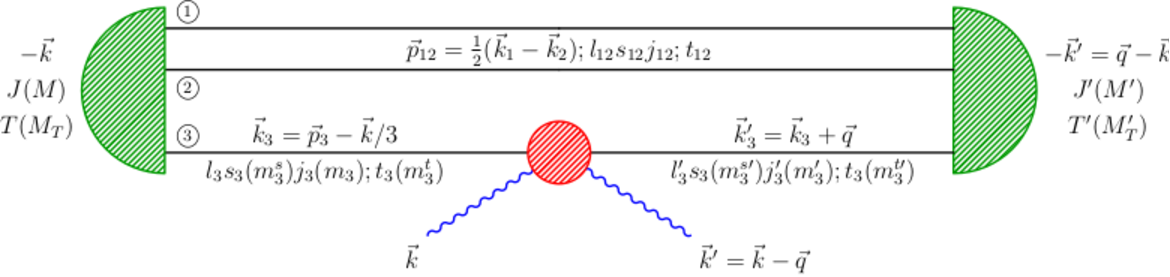
\includegraphics[scale=0.08]{kinematics3He-1bod.png}\\~\\
\end{center}
1 body contribution with $\kt{\alpha}=\kt{[(l_{12}s_{12})\jrel(l_3 s_3)j_3] JM  \sepp(t_{12}t_3)TM_T}$
\begin{equation*}
\begin{split}
    \br{ M '} \, &\hat O_{3} (\kv,\qv) \,\kt{M}
  = \sum_{\alpha \alpha'} \int \dd p_{12}% p_{12}^{2}\;
  \dd{p_{3}} p_{3}^{2} \dd{p_{12}'} p_{12}^{\prime\, 2}
  \dd{p_{3}'} p_{3}^{\prime \, 2}\;
  \psi^{\dagger}_{\alpha'}(p_{12}'p_{3}')   \psi_{\alpha}(p_{12}p_{3})\\ 
  & \times \big\bra \, p_{12}' p_{3}' \left[ (l_{12}' s_{12}')\jrel'
    (l_{3}' s_3) j_{3}' \right] J' M' (t_{12}' t_3 ) T' M_{T} \, \big| \,
  \hat O_{3}(\kv,\qv) \, \\
  &\hspace*{10ex}\big| \, p_{12}p_{3} \left[ (l_{12}
    s_{12})\jrel (l_{3} s_3) j_{3} \right] J M (t_{12} t_3) T M_{T}
  \big\ket  
\end{split}
\end{equation*}
Probe kernel: $\hat{O}_{3}$ changes quantum numbers of active nucleons\\
\end{frame}
%%%%%%%%%%%%%%%%%%%%%%%%%%%%%%%%%%%%%%%%%%%%%%%%%%%%%%%%%%%%%%%%%%%%%%%%%%%%%%%%%%%%%%%%%%%%%%%%%%%

\begin{frame}[fragile]{Details - 1 body}
\begin{center}
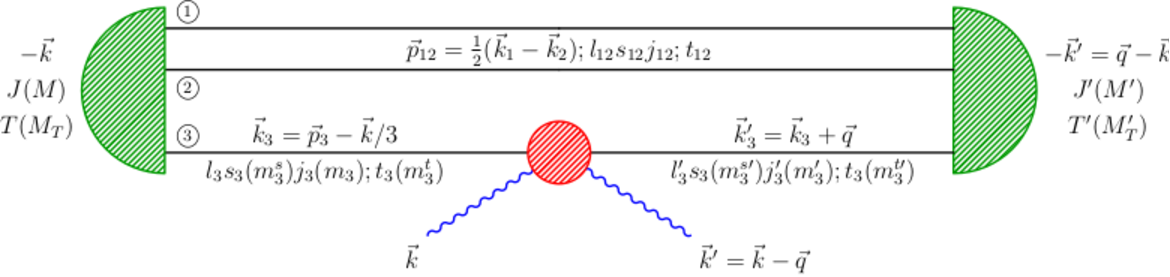
\includegraphics[scale=0.07]{kinematics3He-1bod.png}\\~\\
\end{center}
1 body contribution:
\begin{align*}
    \left\langle M^{\prime}\left|\hat{O}_{3}(\bv{k}, \bv{q})\right| M\right\rangle=\sum_{\substack{m_{3}^{s \prime}\, m_{3}^{s}\\m_3^t}}\hat{O}_{3}\left(m_{3}^{s \prime} m_{3}^{s}, m_{3}^{t} ;  \bv{k}, \bv{q}\right) \rho_{m_{3}^{s \prime} m_{3}^{s}}^{m_3^{t} M_{T}, M^{\prime} M}(\bv{k}, \bv{q})
\end{align*}
Example: Pion Photoproduction: $\hat{O}_3=\frac{1}{2} \vec{ \varepsilon}\cdot \vec{\sigma}_1$
\begin{verbatim}
do i=1, maxI
    rho=readRho(i)
    Result(Mz,Mzp)+= 0.5* rho*sigmax(m1p,m1)
end do
\end{verbatim}
% Probe kernel: $\hat{O}_{3}$ quantum numbers of active nucleons change\\~\\
% Density: $\rho_{m_{3}^{s \prime} m_{3}^{s}}^{m_3^{t} M_{T}, M^{\prime} M}$ involves spectator nucleons
\end{frame}
%%%%%%%%%%%%%%%%%%%%%%%%%%%%%%%%%%%%%%%%%%%%%%%%%%%%%%%%%%%%%%%%%%%%%%%%%%%%%%%%%%%%%%%%%%%%%%%%%%%

%\begin{frame}[fragile]
%\frametitle{One body Implementation}

%\begin{center}
%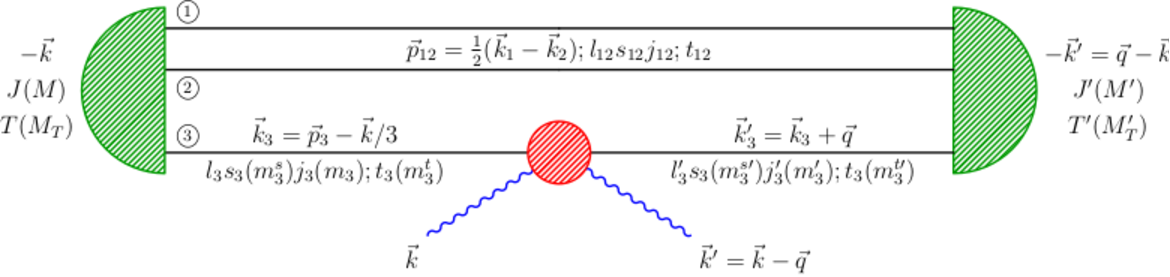
\includegraphics[scale=0.08]{kinematics3He-1bod.png}\\~\\
%\end{center}
%\begin{equation*}
%    \frac{A}{2}\br{M_J'} \vec{ \varepsilon}\cdot \vec{\sigma}_1 \kt{M_J}
%\end{equation*}
%\begin{verbatim}
%do i=1, maxI
%    rho=readRho(i)
%    Result(Mz,Mzp)+= 0.5* A*rho*sigmax(m1p,m1)
%end do
%\end{verbatim}
%\end{frame}
%%%%%%%%%%%%%%%%%%%%%%%%%%%%%%%%%%%%%%%%%%%%%%%%%%%%%%%%%%%%%%%%%%%%%%%%%%%%%%%%%%%%%%%%%%%%%%%%%%%%





\begin{frame}{Details - 2 Body}
\begin{center}
    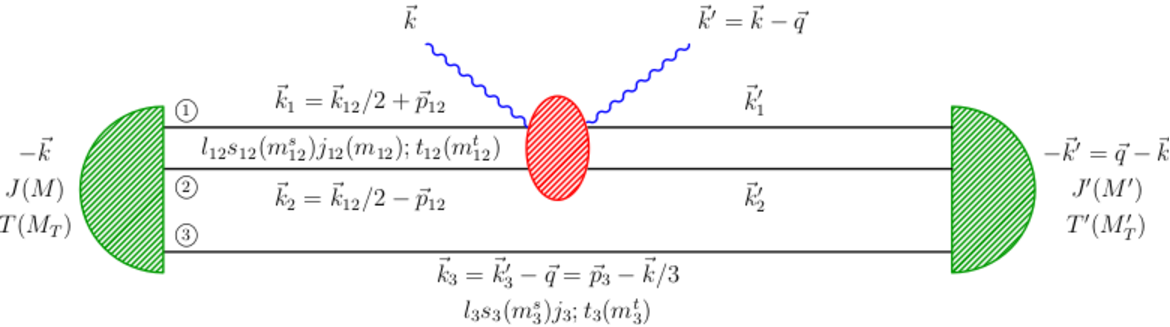
\includegraphics[scale=0.08]{kinematics3He-2bod.png}
\end{center}
\begin{align*}
    \left\langle M^{\prime}\left|\hat{O}_{12}\right| M\right\rangle = \sum_{\alpha_{11}^{\prime}, \alpha_{12}} \int \mathrm{d} p_{12}\:& p_{12}^{2} \mathrm{~d} p_{12}^{\prime}\: p_{12}^{\prime 2}\; O_{12}^{\alpha_{12}^{\prime} \alpha_{12}}\left(p_{12}^{\prime}, p_{12}\right)\nonumber \\
    &\times\rho_{\alpha_{12}^{\prime} \alpha_{12}}^{M_{T}, M^{\prime} M}\left(p_{12}^{\prime}, p_{12} ; \bv{q}\right)
\end{align*}
Relative angular momentum $\ell_{12}$ goes into $\alpha_{12}$\\
Probe kernel: $\hat{O}_{12}$ changes quantum numbers of active nucleons\\~\\
Density: $\rho_{\alpha_{12}^{\prime} \alpha_{12}}^{M_{T}, M^{\prime} M}$ involves only spectator nucleons
\end{frame}
%%%%%%%%%%%%%%%%%%%%%%%%%%%%%%%%%%%%%%%%%%%%%%%%%%%%%%%%%%%%%%%%%%%%%%%%%%%%%%%%%%%%%%%%%%%%%%%%%%%



\begin{frame}
\begin{center}
    Same kernel convolution code can be used with different target densities\\~\\
    Swapping out densities of different targets is trivial
\end{center}
\end{frame}
%%%%%%%%%%%%%%%%%%%%%%%%%%%%%%%%%%%%%%%%%%%%%%%%%%%%%%%%%%%%%%%%%%%%%%%%%%%%%%%%%%%%%%%%%%%%%%%%%%%



\begin{frame}\frametitle{Potentials}
Use potentials to calculate densities\\~\\
We use $\chi$SMS potential  with NN at N4LO and 3N at N2LO and with cutoffs of 400 $\mathrm{MeV}$ and 550 $\mathrm{MeV}$\\~\\
\footn{H. Krebs P. Reinert and E. Epelbaum. “Semilocal momentum-space regularized chiral two-nucleon potentials up to fifth order"}
\end{frame}
%%%%%%%%%%%%%%%%%%%%%%%%%%%%%%%%%%%%%%%%%%%%%%%%%%%%%%%%%%%%%%%%%%%%%%%%%%%%%%%%%%%%%%%%%%%%%%%%%%%






\begin{frame}{2. SRG evolution}{SRG - Similarity Renormalization Group}
\begin{center}
    
My work: $A\leq6$, with $\LiS$, many body interactions much more complicated\\ $\implies$ Density calculation more efficient with SRG evolution.
\end{center}
\footn{See reviews:}
\footn{ Kai Hebeler ``Momentum space evolution of chiral three-nucleon forces" arXiv:1201.0169}
\footn{Sergio Szpigel ``The Similarity Renormalization Group" arXiv:hep-ph/0009071}
\end{frame}
%%%%%%%%%%%%%%%%%%%%%%%%%%%%%%%%%%%%%%%%%%%%%%%%%%%%%%%%%%%%%%%%%%%%%%%%%%%%%%%%%%%%%%%%%%%%%%%%%%%




\begin{frame}\frametitle{Defining an SRG transform}
\begin{center}
Strong dependence on high momentum\\  $\implies$ Difficult numerics for $A>3$\\
\end{center}
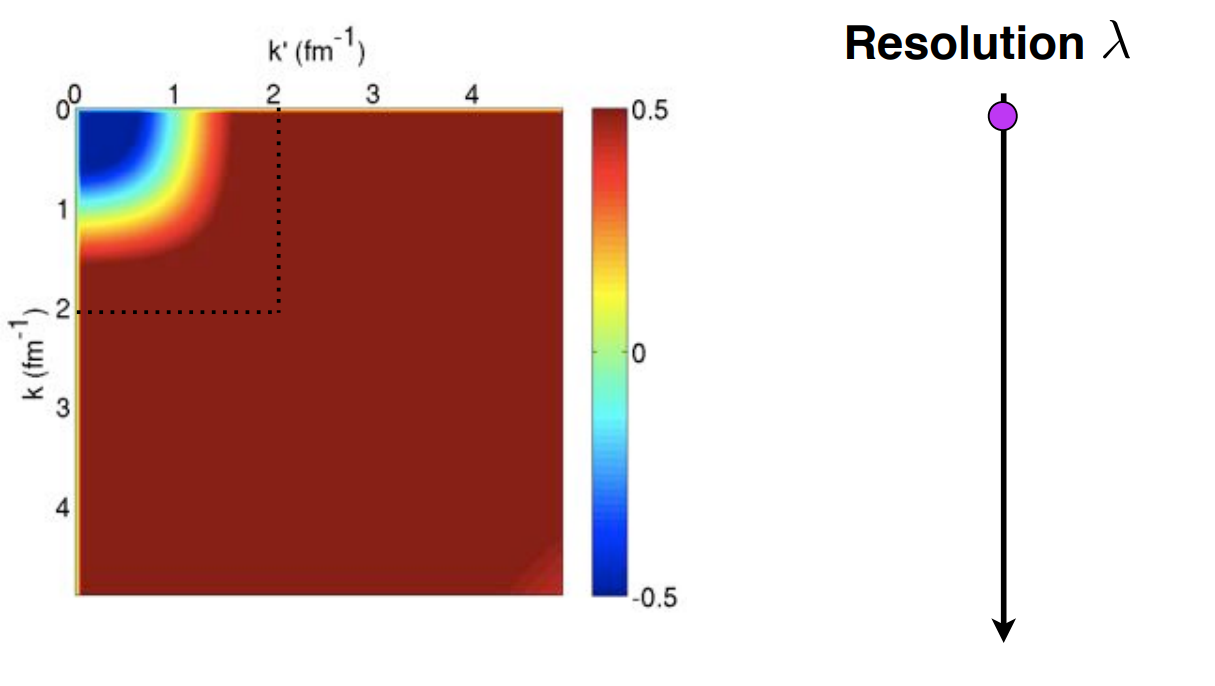
\includegraphics[scale=0.35]{LowRes.png}
\footn{Figures from Kai Hebeler: ``Chiral Effective Field Theory and Nuclear Forces:
overview and applications'' presentation at TALENT school at MITP 2022}
\footn{~\\}
\end{frame}
%%%%%%%%%%%%%%%%%%%%%%%%%%%%%%%%%%%%%%%%%%%%%%%%%%%%%%%%%%%%%%%%%%%%%%%%%%%%%%%%%%%%%%%%%%%%%%%%%%%




\begin{frame}\frametitle{}
\begin{center}
    SRG - shovels all dependence into lower momenta\\~\\
    Medium resolution 
\end{center}
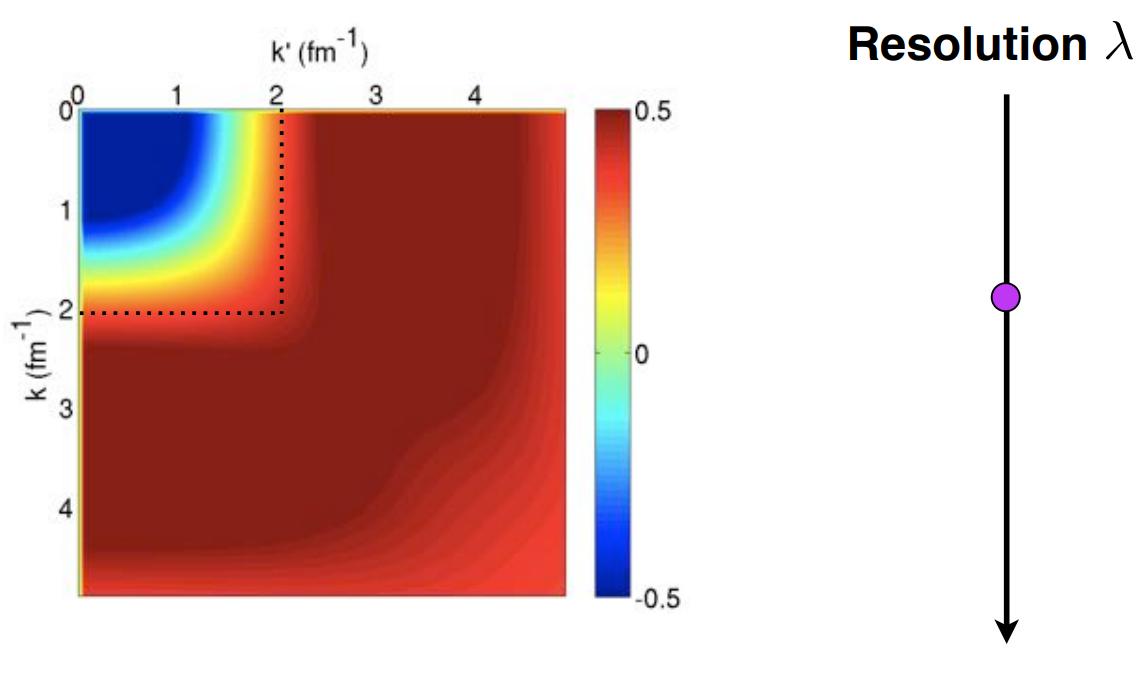
\includegraphics[scale=0.4]{MedRes.png}
\footn{Figures from Kai Hebeler: ``Chiral Effective Field Theory and Nuclear Forces:
overview and applications'' presentation at TALENT school at MITP 2022}
\footn{~\\}
\end{frame}
%%%%%%%%%%%%%%%%%%%%%%%%%%%%%%%%%%%%%%%%%%%%%%%%%%%%%%%%%%%%%%%%%%%%%%%%%%%%%%%%%%%%%%%%%%%%%%%%%%%




\begin{frame}\frametitle{}
\begin{center}
    Low resolution
\end{center}
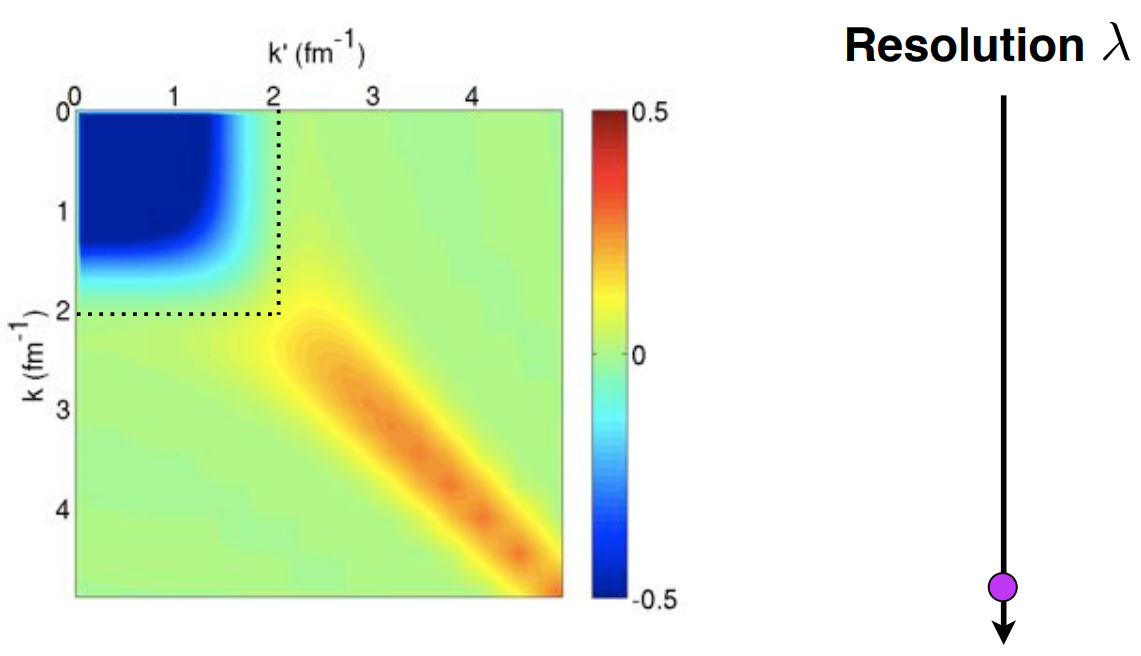
\includegraphics[scale=0.35]{HighRes.png}
~\\
Approximate - cut the potential, only use dependence with $k<2 \mathrm{fm}^{-1}$.\\
Neglects higher order contributions (4 and 5 nucleon etc).\\
Allows for calculation with less ``area" of the potential used\\
Allows $\LiS$ calculation
\end{frame}
%%%%%%%%%%%%%%%%%%%%%%%%%%%%%%%%%%%%%%%%%%%%%%%%%%%%%%%%%%%%%%%%%%%%%%%%%%%%%%%%%%%%%%%%%%%%%%%%%%%




\begin{frame}\frametitle{SRG vs Fourier Transform}
Fourier transforms are discrete unitary transformations
\begin{align*}
    V(\vec{r},\vec{r}\,')&= \br{r'} V \kt{r}\\
                         &= \int \dd^3p\, \dd^3p' \brkt{r'}{p'} \br{p'}V\kt{p} \brkt{p}{r}\\
                         &= V(\vec{p},\vec{p}\,')
\end{align*}
After the transform our free variables have different physical meaning.\\
SRG is similar and it creates problems
\end{frame}
%%%%%%%%%%%%%%%%%%%%%%%%%%%%%%%%%%%%%%%%%%%%%%%%%%%%%%%%%%%%%%%%%%%%%%%%%%%%%%%%%%%%%%%%%%%%%%%%%%%




\begin{frame}{SRG Variables}
Any unitary transform, also transforms the coordinates
\begin{align*}
    \br{p'}V\kt{p} &= \br{p'} \mathbbm{1} V \mathbbm{1} \kt{p}\\
                   &= \br{p'} U^\dag U V U^\dag U \kt{p}\\
                   &= \left(\br{p'} U^\dag\right)\;\left( U V U^\dag\right)\;\left( U \kt{p}\right)\\
                   &= \br{\widetilde{p}\,'} V_{eff} \kt{\widetilde{p}}
\end{align*}
Calling the free parameters in the SRG potential ``momenta" is abuse of notation. They are not physical momenta.
\end{frame}
%%%%%%%%%%%%%%%%%%%%%%%%%%%%%%%%%%%%%%%%%%%%%%%%%%%%%%%%%%%%%%%%%%%%%%%%%%%%%%%%%%%%%%%%%%%%%%%%%%%




\begin{frame}\frametitle{Density Calculation}
SRG changes Hamiltonian $\implies$ changes Lagrangian $\implies$ diagram contribution changes, and momenta aren't
physical\\~\\
One option: do a unitary transform of diagrams and kernels
\begin{center}
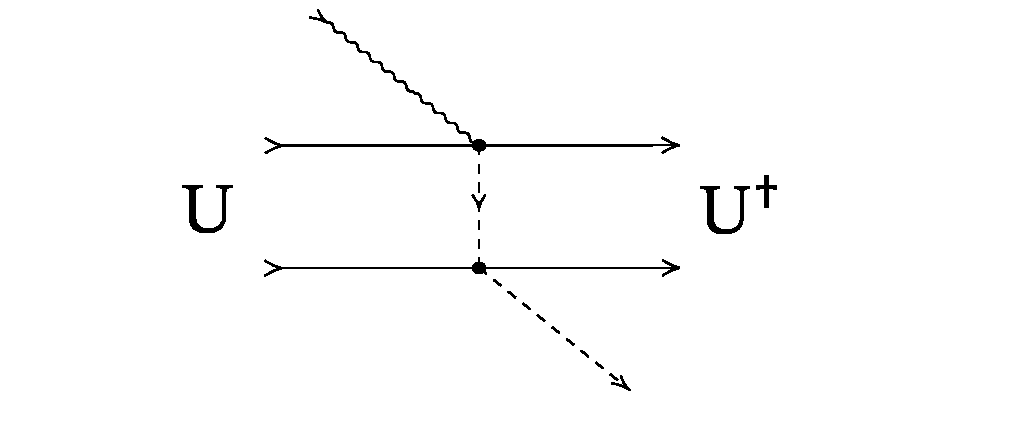
\includegraphics[scale=0.5]{UUdag.pdf}
\end{center}
Problem: This breaks kernel - target (density) independence. Would have to introduce SRG $\lambda$ dependence into the code\\
\qquad - Effectively would give SRG dependence on Lagrangian and therefore the diagrams.
\end{frame}
%%%%%%%%%%%%%%%%%%%%%%%%%%%%%%%%%%%%%%%%%%%%%%%%%%%%%%%%%%%%%%%%%%%%%%%%%%%%%%%%%%%%%%%%%%%%%%%%%%%




\begin{frame}{3. Specific Systems}{Initial $\HeF$}
$\HeF$ Compton scattering, with and without SRG
\begin{center}
    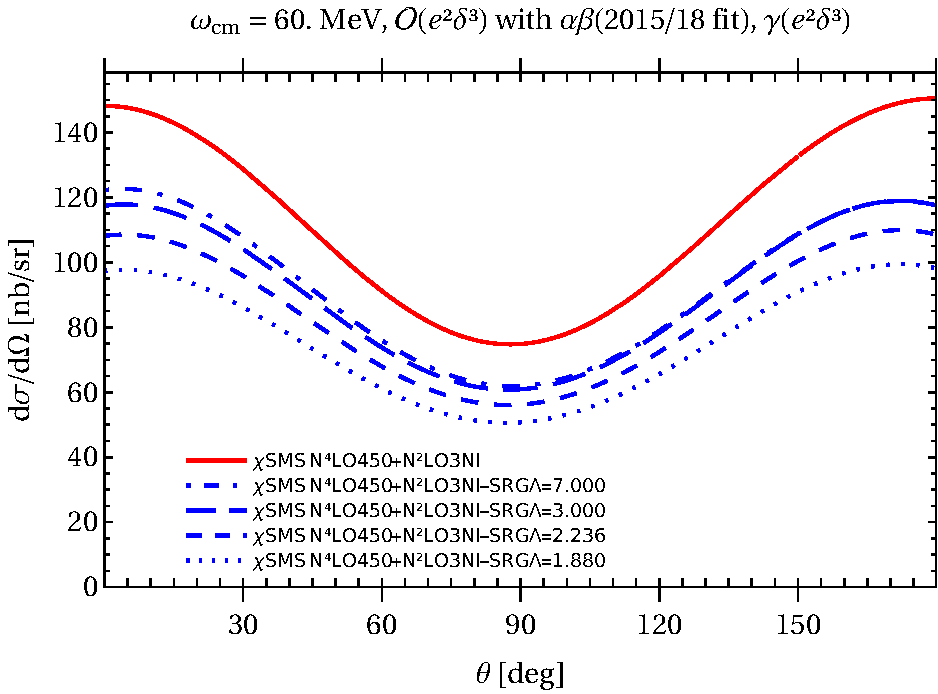
\includegraphics[scale=0.5]{4HeSRGCompare.pdf}
\end{center}
Smaller $\lambda \Rightarrow$ more change $\Rightarrow $ further deviation from true value
\end{frame}
%%%%%%%%%%%%%%%%%%%%%%%%%%%%%%%%%%%%%%%%%%%%%%%%%%%%%%%%%%%%%%%%%%%%%%%%%%%%%%%%%%%%%%%%%%%%%%%%%%%






\begin{frame}\frametitle{Initial $\LiS$ }
\begin{center}
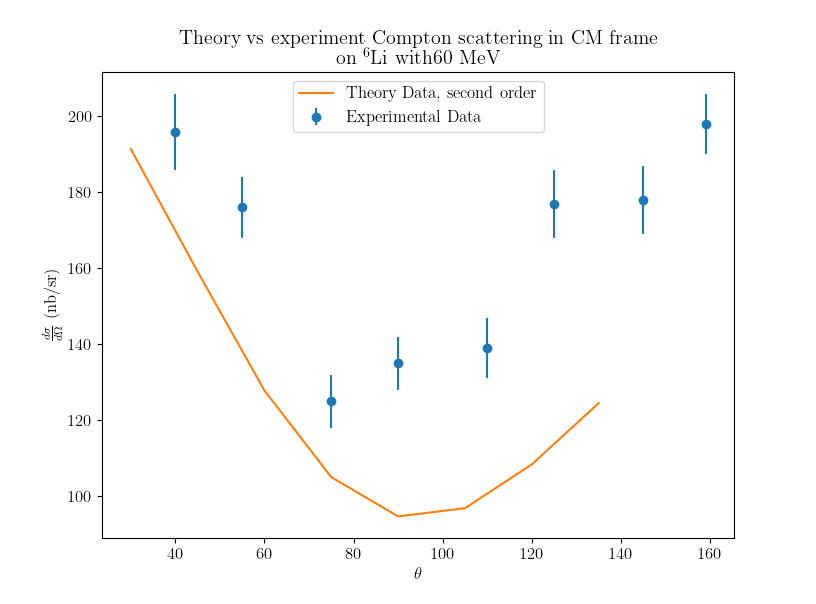
\includegraphics[scale=0.5]{Li6Result1.png}
\end{center}
\end{frame}
%%%%%%%%%%%%%%%%%%%%%%%%%%%%%%%%%%%%%%%%%%%%%%%%%%%%%%%%%%%%%%%%%%%%%%%%%%%%%%%%%%%%%%%%%%%%%%%%%%%






\begin{frame}\frametitle{Density Calculation}
\begin{itemize}
    \item Transforming the diagrams against the philosophy of separating the kernel from the target
    \item Instead: Back transform the densities 
\end{itemize}
~\\Xiang-Xiang Sun and Andreas Nogga have completed the back transform, with our collaboration (to be published).\\~\\
Have $\HeF$ with and without SRG back transform for comparison \\~\\
Gained confidence moving $\LiS$

\end{frame}
%%%%%%%%%%%%%%%%%%%%%%%%%%%%%%%%%%%%%%%%%%%%%%%%%%%%%%%%%%%%%%%%%%%%%%%%%%%%%%%%%%%%%%%%%%%%%%%%%%%




\begin{frame}{Comparison - Compton Scattering Results on $\HeF$}
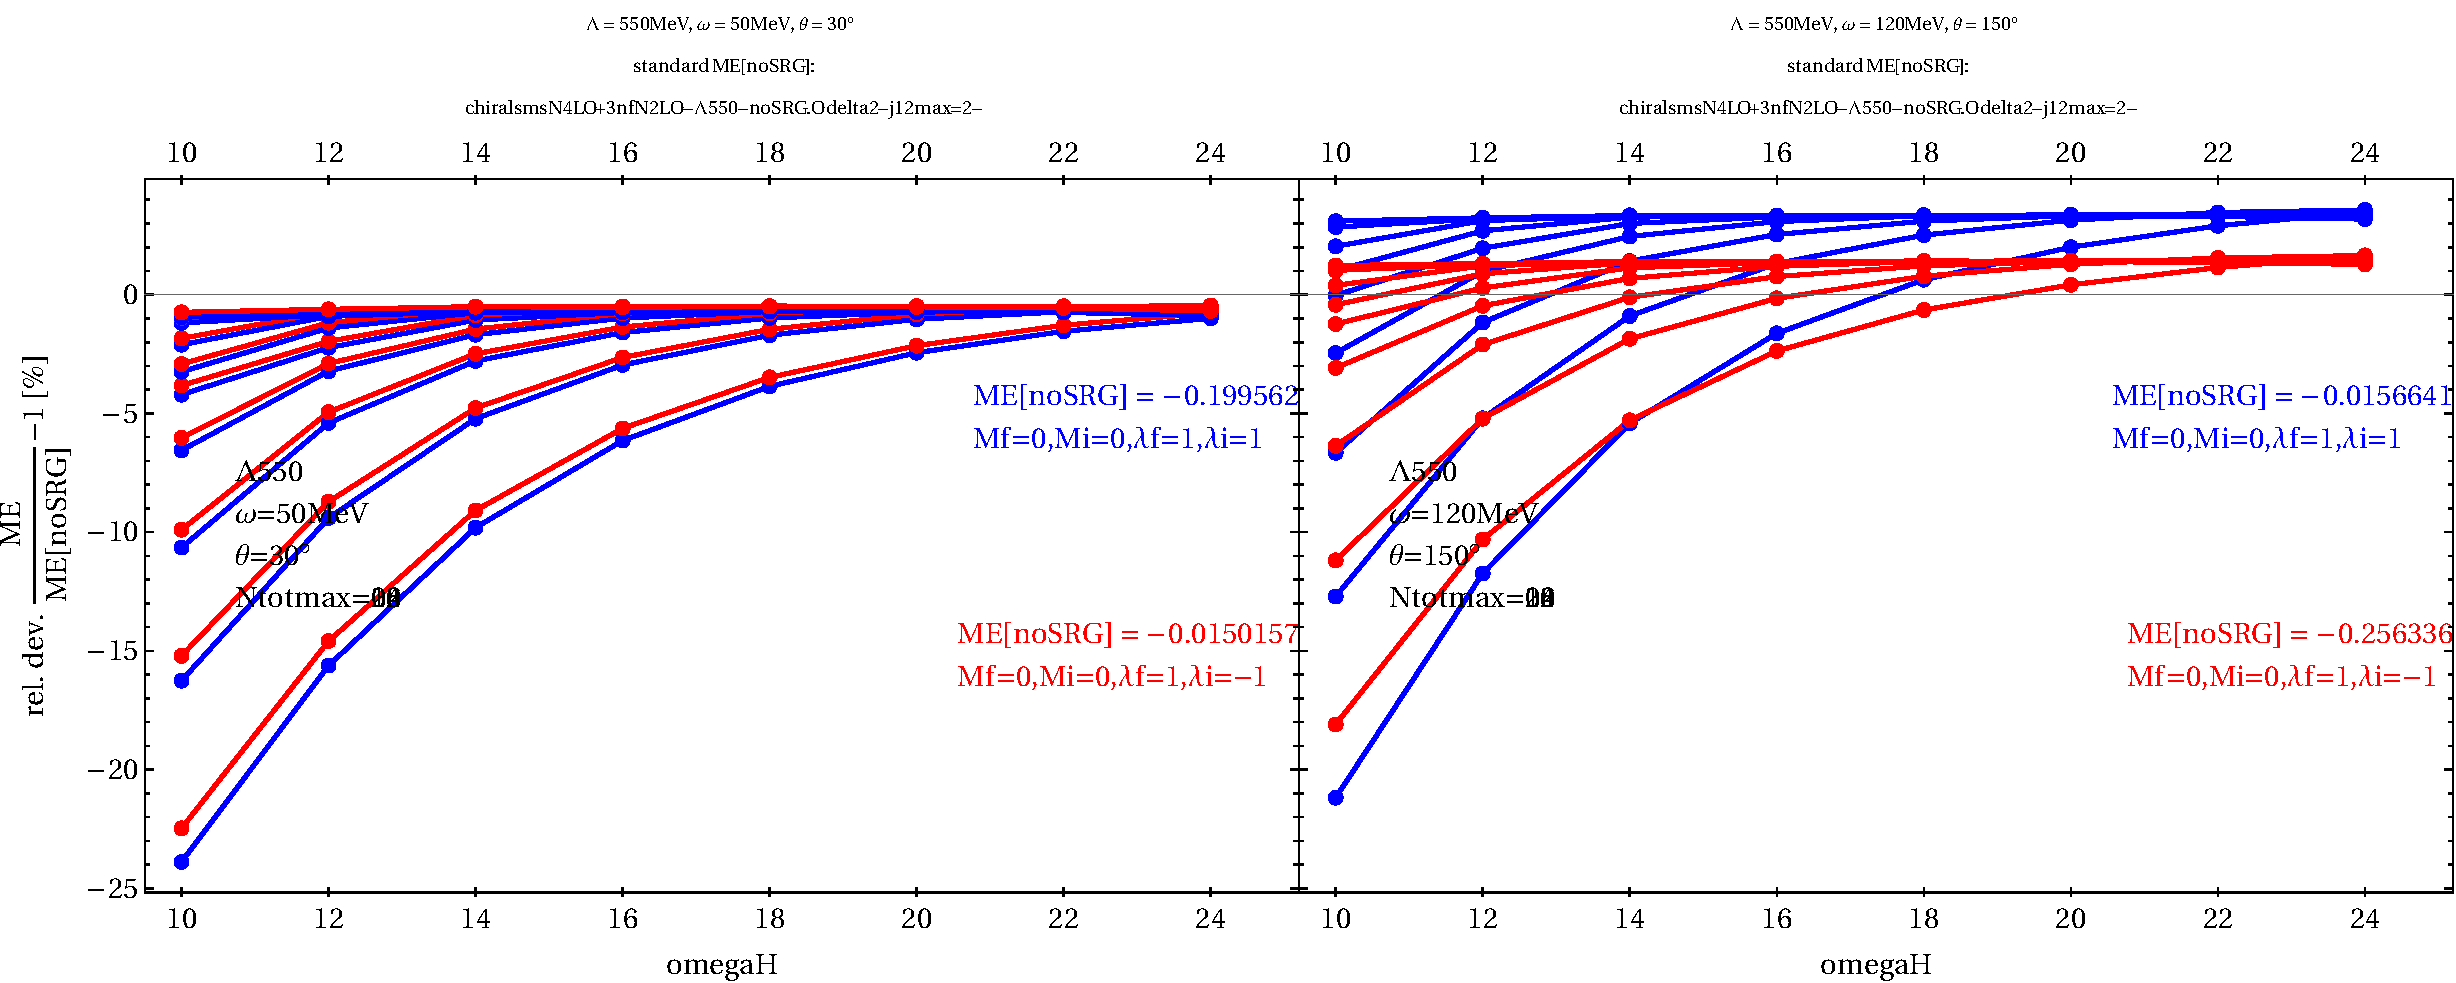
\includegraphics[scale=0.28]{SRG-Converge-Double.pdf}
SRG calculation uses harmonic oscillator basis, non-SRG uses Fadeev basis\\
Differences come from SRG induced many body forces and difference in basis\\
Each line: different maximum of number of states\\
$x$-axis: width of harmonic oscillator potential 
\end{frame}
%%%%%%%%%%%%%%%%%%%%%%%%%%%%%%%%%%%%%%%%%%%%%%%%%%%%%%%%%%%%%%%%%%%%%%%%%%%%%%%%%%%%%%%%%%%%%%%%%%%







\begin{frame}\frametitle{Reactions}
$\gamma X \to \gamma X$\\
Already implemented, can do new targets\\~\\

$\gamma X \to \pi^0 X$\\
Technical limitation $\implies$ require $\pi^0$\\
Initial kernel: Beane/... NPA 618(1997) 381\\
~\\
$\pi X \to \pi X$\\ Charged pions $\implies$ easier for experiment\\
Initial considerations: Beane/... NPA 720(2003) 399\\~\\
\end{frame}
%%%%%%%%%%%%%%%%%%%%%%%%%%%%%%%%%%%%%%%%%%%%%%%%%%%%%%%%%%%%%%%%%%%%%%%%%%%%%%%%%%%%%%%%%%%%%%%%%%%



\begin{frame}\frametitle{Kernel Similarity}
\begin{center}
\begin{figure}
\includegraphics[scale=0.35]{Topology2.png}

\caption{Two body kernels for: Top - Compton scattering; Middle - Pion scattering; Bottom - pion photoproduction}
\end{figure}
\end{center}
\end{frame}
%%%%%%%%%%%%%%%%%%%%%%%%%%%%%%%%%%%%%%%%%%%%%%%%%%%%%%%%%%%%%%%%%%%%%%%%%%%%%%%%%%%%%%%%%%%%%%%%%%%






\begin{frame}\frametitle{Specific Systems}
\begin{center}
    Technical limitation $\implies$ nucleus doesn't change\\~\\
    Reactions are $yX \to zX$ with \\~\\
    $X= \HeT, \HeF, {}^3 \mathrm{H}, \LiS$\\~\\
\end{center}
\end{frame}
%%%%%%%%%%%%%%%%%%%%%%%%%%%%%%%%%%%%%%%%%%%%%%%%%%%%%%%%%%%%%%%%%%%%%%%%%%%%%%%%%%%%%%%%%%%%%%%%%%%



\begin{frame}\frametitle{Extraction - Compton Scattering $\gamma X \to \gamma X$} 
\begin{columns}
    \begin{column}{.5\textwidth}
    Feldman, Downie: $\gamma \LiS \to \gamma \LiS$\\~\\
    Extract nucleon polarizabilities $\alpha_{E1}$ and $\beta_{M1}$ (stiffness)\\~\\

    $\mathcal{H}=-4\pi \left( \frac{1}{2} \alpha_{E1} \bv{E}^2 + \frac{1}{2} \beta_{M1} \bv{H}^2\right)$.\\~\\
    Many experiments on $\LiS$, no theory prediction \\~\\
    Kernel exists and is implemented\\
    % Need $\LiS$ density\\
    % $\HeF$ currently being written, will be on arXiv before January 31st
    \end{column}
% create the column with the second image, that also
% occupies half of the slide
    \begin{column}{.5\textwidth}
    \begin{figure}
    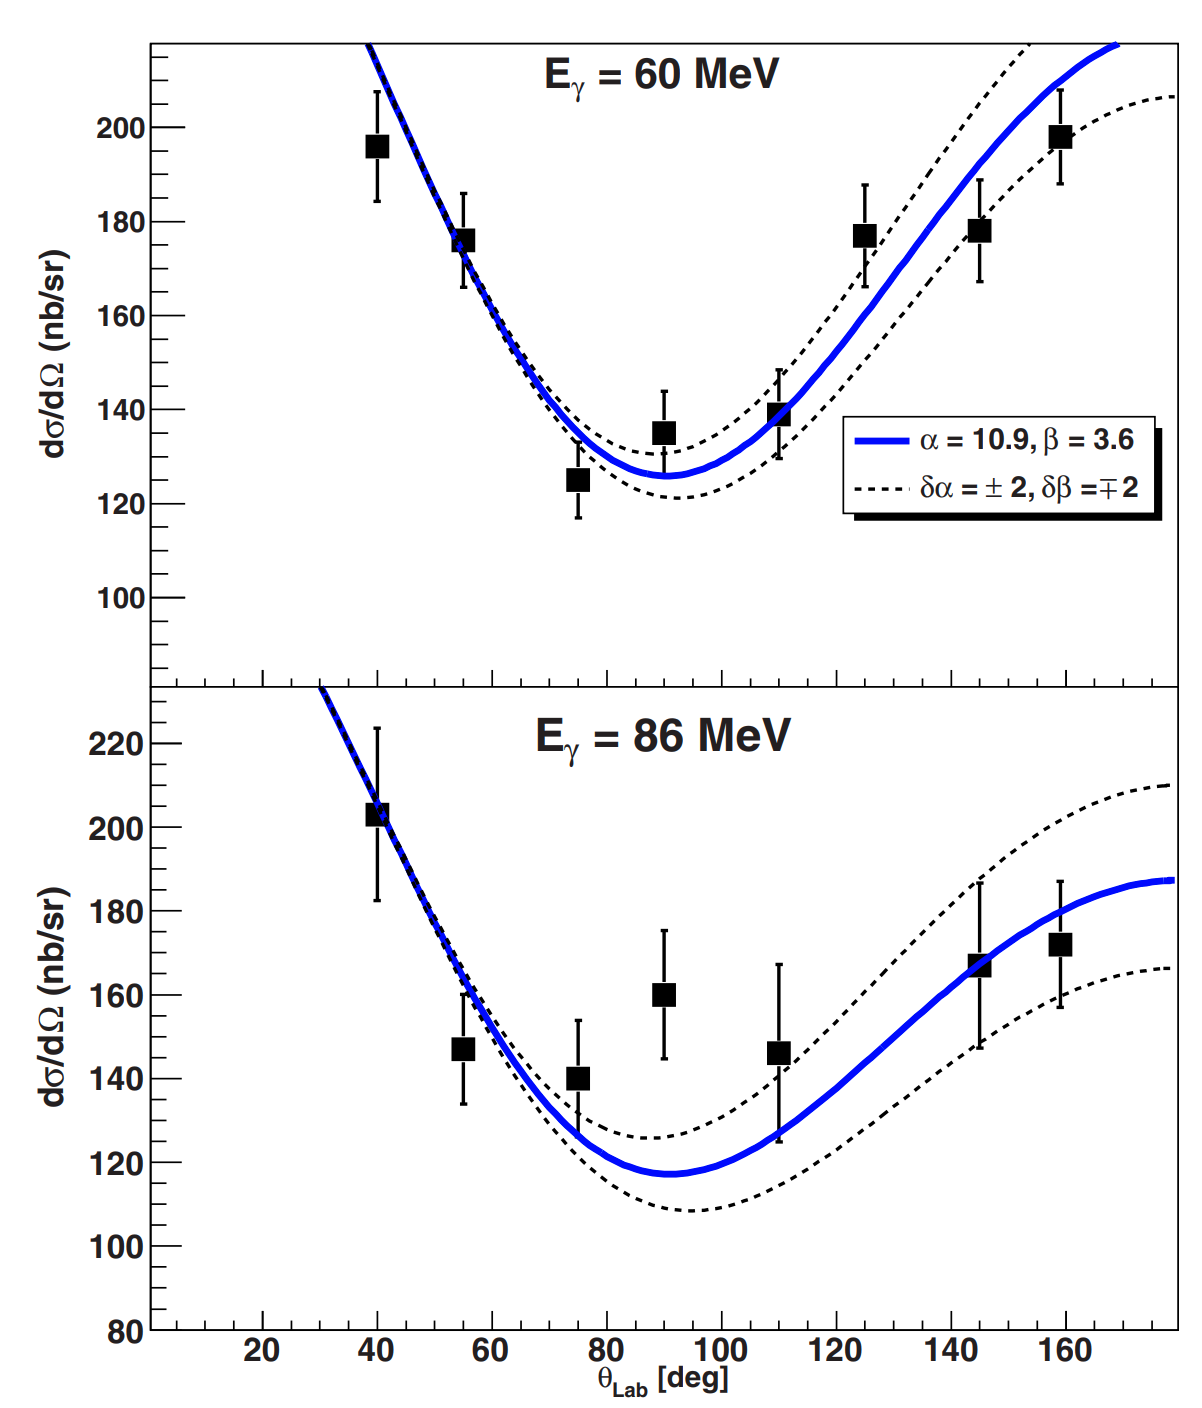
\includegraphics[width=0.8\textwidth]{Li6Feldman.png}
    \caption{Myers/... PRC 90(2014) 027603}
    \end{figure}
    \end{column}
\end{columns}
\end{frame}
%%%%%%%%%%%%%%%%%%%%%%%%%%%%%%%%%%%%%%%%%%%%%%%%%%%%%%%%%%%%%%%%%%%%%%%%%%%%%%%%%%%%%%%%%%%%%%%%%%%




%\begin{frame}\frametitle{$\LiS$ result}
%INSERT RESULTS HERE ONCE WE HAVE THEM
%\end{frame}
%%%%%%%%%%%%%%%%%%%%%%%%%%%%%%%%%%%%%%%%%%%%%%%%%%%%%%%%%%%%%%%%%%%%%%%%%%%%%%%%%%%%%%%%%%%%%%%%%%%%




%\begin{frame}\frametitle{Pion Photoproduction}
%First one body diagram, at threshold:
%\begin{center}
%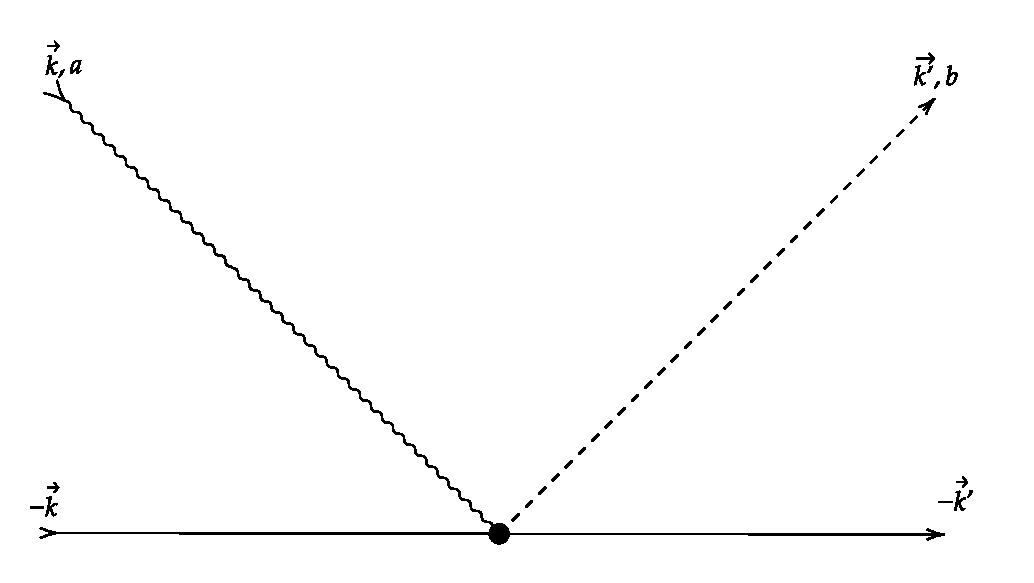
\includegraphics[scale=0.4]{1A.pdf}
%\end{center}

%\begin{equation*}
%    \frac{A}{2}\br{M_J'} \vec{ \varepsilon}\cdot \vec{\sigma}_1 \kt{M_J}
%\end{equation*}
%\end{frame}
%%%%%%%%%%%%%%%%%%%%%%%%%%%%%%%%%%%%%%%%%%%%%%%%%%%%%%%%%%%%%%%%%%%%%%%%%%%%%%%%%%%%%%%%%%%%%%%%%%%%




%\begin{frame}[fragile]
%\frametitle{One body Implementation}

%\begin{equation*}
%    \frac{A}{2}\br{M_J'} \vec{ \varepsilon}\cdot \vec{\sigma}_1 \kt{M_J}
%\end{equation*}
%\begin{verbatim}
%do i=1, maxI
%    rho=readRho(i)
%    Result(Mz,Mzp)+= 0.5* A*rho*sigmax(m1p,m1)
%end do
%\end{verbatim}
%\end{frame}
%%%%%%%%%%%%%%%%%%%%%%%%%%%%%%%%%%%%%%%%%%%%%%%%%%%%%%%%%%%%%%%%%%%%%%%%%%%%%%%%%%%%%%%%%%%%%%%%%%%%


\begin{frame}\frametitle{Two body Pion Photoproduction}
\begin{center}
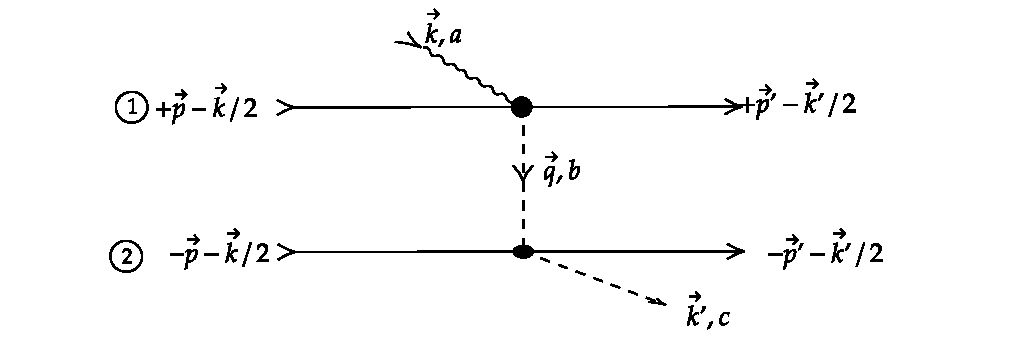
\includegraphics[scale=0.6]{pionphoto-2A.pdf}\\
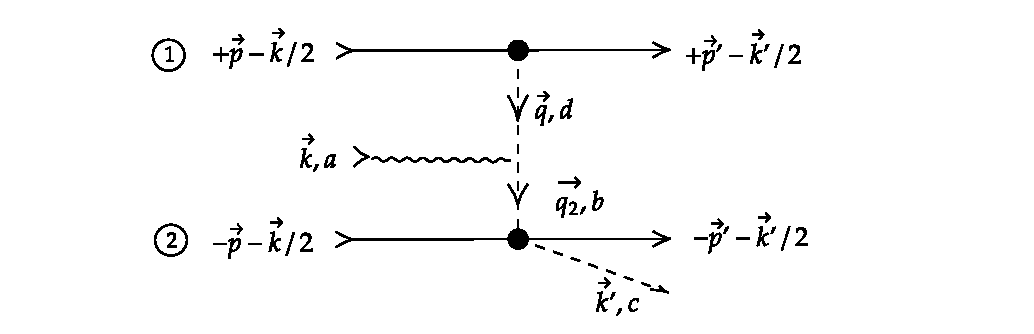
\includegraphics[scale=0.6]{pionphoto-2B.pdf}
\end{center}
\end{frame}
%%%%%%%%%%%%%%%%%%%%%%%%%%%%%%%%%%%%%%%%%%%%%%%%%%%%%%%%%%%%%%%%%%%%%%%%%%%%%%%%%%%%%%%%%%%%%%%%%%%





\begin{frame}\frametitle{Pion Photoproduction Two Body Result - At threshold}
Lenkewitz Result arXiv:1103.3400 
\begin{align*}
    &\text{Lenkewitz (AV18+UIX) } &\text{My Result (CHSMS)}\\
    x,y\; \text{polarization}:& -29.3 \;\mathrm{fm}^{-1}& \sim-31\; \mathrm{fm}^{-1}\\
    z\; \text{polarization}:& -22.9\; \mathrm{fm}^{-1}&\sim-24\; \mathrm{fm}^{-1}\\
\end{align*}
\%6.6  and \%5.3 difference\\~\\
My result is currently numerically unstable

\end{frame}
%%%%%%%%%%%%%%%%%%%%%%%%%%%%%%%%%%%%%%%%%%%%%%%%%%%%%%%%%%%%%%%%%%%%%%%%%%%%%%%%%%%%%%%%%%%%%%%%%%%




\begin{frame}\frametitle{Conclusion}
\begin{itemize}
\item Kernel, for $\gamma X \to \gamma X$, $\gamma X \to \pi X$, $\pi X \to \pi X$
\begin{itemize}
    \item Development
    \item Coding
    \item Convolution
\end{itemize}
~\\
\item Extract, predict, and parameterize scattering processes\\~\\
\item Fill in theory gap for experiment\\~\\
\item Lay groundwork for future work with densities
\begin{itemize}
    \item So far has only been used with Compton, and dark matter scattering
    \item Trigger interest: J. de Vries et. al. ``Dark matter scattering off $\HeF$ in chiral effective field theory"\\
        \href{https://arxiv:2310.11343}{arxiv:2310.11343}
\end{itemize}
\end{itemize}
\end{frame}
%%%%%%%%%%%%%%%%%%%%%%%%%%%%%%%%%%%%%%%%%%%%%%%%%%%%%%%%%%%%%%%%%%%%%%%%%%%%%%%%%%%%%%%%%%%%%%%%%%%




\end{document}
